In this section we explore some ideas of how to study properties of quantum graphs and introduce concepts that will be play a central role in \cref{sec: snowflake}.



\section{Physical phenomena represented by the vertex conditions}\label{sec: physical interpretation mc}

In quantum mechanics, the wave function $\psi$ is required to be continuous and continuously differentiable (for finite potentials), i.e.\ $\psi \in C^1$. The function must also be normalizable, i.e.\ $\psi \in L^2$, to satisfy the requirement that the total probability of detecting the particle \emph{anywhere} equals unity, that is
\[
  \int \abs{\psi}^2 dx = 1.
\]
The normalizability condition can in some sense be weakened for semi-infinite edges, we will return to this when we encounter such graphs. What remains is then to consider how the wave function behaves at the vertices, and what requirements to impose so that the graph properly reflects the physics. In section~\ref{sec: mc} we introduced the standard matching conditions and showed why it is natural to impose such conditions from a physical point of view. We will now explore other vertex conditions and through various examples see how they reflect the physics at play.

It is instructive, both for the readers already familiar with the basics of quantum mechanics and for those who are not, to consider the classical example of a particle in a box in the language of quantum graphs.


\begin{example}[Finite line graph with Dirichlet conditions: particle in a box]\label{ex: particle in a box}
  The problem constitutes of finding the stationary states of a quantum mechanical particle confined in a one-dimensional box with impenetrable walls, i.e.\ an infinitely strong potential outside the boundary of the box. Inside the box, represented as an interval parametrized from 0 to $\ell$, the particle propagates freely, c.f.\ figure~\ref{fig: finite line graph}.

  \begin{figure}[!h]
   \centering
    \begin{tikzpicture}[vertex/.style={draw,circle,minimum size=1.3mm,inner sep=0pt,outer sep=0pt,fill=black},scale=4]
      \draw (0, 0) -- (1, 0);
      \node[vertex] at (0, 0) {};
      \node[vertex] at (1, 0) {};
      \node[below] at (0, 0) {$0$};
      \node[below] at (1, 0) {$\ell$};
    \end{tikzpicture}
    \caption{Finite line graph of length $\ell$, parametrized from $0$ to $\ell$.}
    \label{fig: finite line graph}
  \end{figure}

  This example illustrates that the standard matching conditions do not necessarily reflect the physics for the outer vertices, instead one considers the \emph{Dirichlet condition} for the outer vertices $v$,
  \[ u(v) = 0. \]
  When the graph is interpreted as a physical object, the probability of finding the particle outside of the graph is 0, hence the continuity condition actually reduces to the Diriclet condition. Requiring this for every vertex, or only for the outer vertices with standard matching conditions for the inner vertices (if such are present in the graph), clearly causes the boundary terms \ref{eq: mc boundary terms} to vanish, so there exists a self-adjoint extension of $L^{min}$ in this case also.

  Hence, the stationary states with energy $\lambda$ are given by the eigenfunctions $u(x)$ to the Laplace operator satisfying the Diriclet condition. That is,
  \[ Lu(x) = \lambda u(x), \quad u(0) = u(\ell) = 0. \]
  For $\lambda = 0$ we get
  \[ u(x) = ax + b, \quad u(0) = b = 0, \quad u(\ell) = a\ell = 0, \]
  which is just the trivial solution.
  For $\lambda = k^2 > 0$ the general solution is
  \[ u(x) = A \sin kx + B \cos kx. \]
  The vertex condition gives
  \[ u(0) = B = 0 \]
  and then,
  \[ u(\ell) = A \sin k\ell = 0 \]
  With $A=0$ we get the trivial solution, so we require $A \ne 0$, then $k\ell = \pi n$ for $n=1,2,\ldots$. That is, we have the eigenfunctions with corresponding eigenvalues
  % \[ u(x) = A \sin kx, \quad \lambda = k^2 = \frac{\pi^2}{\ell^2}n^2. \tag*{$\blacksquare$} \]
  \[ u(x) = A \sin kx, \quad \lambda = k^2 = \frac{\pi^2}{\ell^2}n^2, n=1,2,\ldots. \]
  Finally the case $\lambda < 0$ is not possible since the operator is positive, this can also be seen by direct calculation.
\end{example}


\begin{example}[Finite line graph with Neumann conditions: waves in a fluid]
  Consider again the line graph described in example~\ref{ex: particle in a box}, but now with standard matching conditions. The continuity condition is trivially satisfied since the vertices have degree 1. The condition on the derivatives reduces to the so called \emph{Neumann condition} at each vertex $v$:
  \[ \partial u(v) = 0. \]
  These conditions correspond to waves in a fluid being reflected from a wall. In this case the eigenfunctions $u(x)$ and eigenvalues $\lambda = k^2 > 0$ of $L$ are given by
  \[ u(x) = A \cos kx, \quad \lambda = k^2 = \frac{\pi^2}{\ell^2}n^2, n=0,1,2,\ldots. \]
  Note that we get different eigenfunctions as example~\ref{ex: particle in a box} while the spectrum is the same, except that one additional point is included in the spectrum when we have Neumann conditions. The ground state is allowed to have zero energy because the constant function $u(x) \equiv 1$ is a solution to $Lu=0$ with Neumann conditions.
\end{example}


Other matching conditions are often studied also for the inner vertices, for example the $\delta$-conditions at vertex $v$, where the condition on the derivatives in the standard matching conditions is changed. The $\delta$-conditions at a vertex $v$ are defined by
\begin{equation}
  \left\lbrace\begin{aligned}
    &u(x) = u(y) \text{ for all } x, y \in v\\
    &\sum_{x \in v} \partial u(x) = \alpha u(v)
  \end{aligned}\right.
\end{equation}
For $\alpha = 0$ we get back the standard matching conditions, so the delta conditions can be seen as a generalization of the standard conditions. These conditions can be shown to represent a Dirac delta potential at the vertex $v$ of strength $\alpha$. Physically this can be seen as an approximation of a graph where the edges consist of conducting material---say thin metal wires---such that the edges are connected at the vertices via some thin non-conducting interface, for example air if the edges are not properly aligned. An electron propagating through this graph will then experience a potential resembling a delta function at the vertices, through which the electron tunnels.

In chapter~\ref{sec: snowflake} we will encounter vertex conditions that do not directly represent any physical phenomenon. However, the graph will be equivalent to a geometrically different graph, in the sense that the two graphs have identical scattering properties.

As we've seen there is an interplay between the geometry of the graph and the vertex conditions, both of which affect the operator of the graph, for example its domain. The line graph that we studied above can be seen as the simplest non-trivial graph, it served well for bridging the gap between the language of quantum mechanics and that of quantum graphs, which was the ambition of this section. In subsequent sections we will encounter graphs of more interesting geometry, for example the star graph considered in section~\ref{sec: star graph} can be seen as a natural generalization of the line graph.




\section{Scattering phenomena and inverse problems}\label{sec: scattering phenomena}

Scattering phenomena are general physical processes where particles, or more generally some form of radiation, is being deflected from its natural trajectory. Scattering can be used to study properties of objects, by sending radiation towards the object and measuring the scattering, i.e.\ the spread, angle and intensity of the deflected radiation. Such problems, where one tries to reconstruct the structure of an object from, are generally called inverse problems. In the context of quantum graphs one consider what can be said about the graph based on known spectral properties or scattering properties.

\begin{figure}[h]
  \centering
  \begin{tikzpicture}[vertex/.style={draw,circle,minimum size=1.3mm,inner sep=0pt,outer sep=0pt,fill=black},scale=0.6]
    \node[vertex] at (0,0) (v0) {};
    \node[vertex] at (3,-2) (v1) {};
    \node[vertex] at (3,2) (v2) {};
    \node[vertex] at (6,0) (v3) {};
    \draw
      (v0) -- (v1)
      (v0) -- (v2)
      (v1) -- (v2)
      (v1) -- (v3)
      (v2) -- (v3);
    \draw[dash pattern=on 5pt off 2pt]
      (-7,1) -- (v0)
      (v2) -- (9,7)
      (v3) -- (12,1);

    \draw[->, thick] (-4.75,{5/7+0.5}) -- (-3.75,{4/7+0.5});
    \draw[->, thick] (-2.25,{2.5/7+0.5}) -- (-3.25,{3.5/7+0.5});
    \draw[->, thick] (5.5,{5/6*5.5-1/2+1/2}) -- (6.5,{5/6*6.5-1/2+1/2});
    \draw[->, thick] (8.5,{1/6*8.5-1+1/2}) -- (9.5,{1/6*9.5-1+1/2});

    \node at (-3.5,{3.5/7-0.5}) {$e_1$};
    \node at (6.3,{5/6*6-1/2-0.5}) {$e_2$};
    \node at (9,{1/6*9-1-0.5}) {$e_3$};

    \node at (-0.2,0.6) {$v_1$};
    \node at (2.7,2.6) {$v_2$};
    \node at (6.2,-0.7) {$v_3$};
  \end{tikzpicture}
  \caption{Scattering from an incoming wave on edge $e_1$.}
  \label{fig: scattering graph}
\end{figure}

Consider the graph in figure~\ref{fig: scattering graph}, the dashed edges should be regarded as ways in to the graph and the vertices $v_1, v_2$ and $v_3$ are the contact points. The figure illustrates how an incoming wave $\psi_1(x) = A_1e^{ikx}+B_1e^{-ikx}$ on edge $e_1$ gets scattered.
If we choose a parametrization for $e_1, e_2$ and $e_3$ directed away from the graph, for example a parametrization from $0$ to $\infty$, the amplitude for the incoming wave on edge $e_i$ is $A_i$ and the amplitude for the outgoing is $B_i$. To take all edges into account at once we define
\[
  \Psi_{in} =
  \begin{pmatrix}
    A_1 \\ A_2 \\ A_3
  \end{pmatrix} e^{ikx}, \quad
  \Psi_{out} =
  \begin{pmatrix}
    B_1 \\ B_2 \\ B_3
  \end{pmatrix} e^{-ikx}.
\]
To completely characterize the scattering from the graph, we need information about how an incoming wave on each of the edges $e_1, e_2$ and $e_3$ is scattered at the graph, that is, how much of the wave that is being reflected and transmitted via the two remaining edges. For this purpose we introduce the $S$-matrix as satisfying the relation
\[
  \Psi_{out} = S \Psi_{in}.
\]
For the graph in figure~\ref{fig: scattering graph} the $S$-matrix is given by
\[
  S =
  \begin{pmatrix}
    S_{11} & S_{12} & S_{13} \\
    S_{21} & S_{22} & S_{23} \\
    S_{31} & S_{32} & S_{33}.
  \end{pmatrix}
\]
Note that for a wave incoming from edge $e_i$ the coefficient $S_{ii}$ is the reflection coefficient, i.e.\ $\abs{S_{ii}}^2$ is the probability of the wave being reflected, and $S_{ji}$ is the transmission coefficient from edge $e_i$ to edge $e_j$, where $j \ne i$.

Recall the discussion on probabilities for quantum states in section~\ref{sec: quantum states and interpretations of quantum mechanics}, the squared modulus of the reflection and transmission coefficients correspond precisely to the probability of a quantum mechanical particle undergoing scattering as described to get reflected or transmitted. Due to
probability conservation we have $\norm{A}^2 = \norm{B}^2$, which means that the $S$-matrix is unitary.

Furthermore, note that the graph in figure~\ref{fig: scattering graph} possesses a mirror symmetry along edge $e_2$, i.e.\ reflecting the graph along the axis given by $e_2$ we get back an equivalent graph, though this is not directly evident from the graphical representation of the graph, as the angle of edge $e_1$ is not preserved. However, a quantum graph is not embedded in any space, there is no concept of angles between edges. Therefore, when we embed a graph in space, when we draw a picture of the graph, the angles between the edges play no role. The drawing in figure~\ref{fig: scattering graph} is intentionally drawn asymmetric to emphasize that symmetries of graphs are not dependent on the graphical representation.

Thus we conclude that, for the graph in figure~\ref{fig: scattering graph}, a wave incoming from $e_1$ propagates through the graph just as a wave incoming from $e_3$ does, after applying the mirror symmetry. Similarly, a wave incoming from edge $e_2$ gets transmitted as much into edges $e_1$ as into edge $e_3$. That is, the scattering coefficients $S_{ij}, i=1,2,3$ are unchanged if, for the indexes $i$ and $j$, $1$ is replaced with $3$ and vice versa.

Symmetries of the graph can often be used to extract information from a graph and to simplify calculations, in the following sections we explore this further and introduce a theorem that will later be useful.



\section{Graph symmetries}\label{sec: graph symmetries}

It can be very difficult to analyze a graph and characterize its properties without paying attention to the graph symmetries. In this section we properly define what is meant by a symmetry of a graph and explore how graph symmetries can be used. As we have seen in chapter~\ref{sec: defining quantum graphs}, the matching conditions reflect the geometry of the underlying graph. However, it is often very useful to directly exploit the symmetries of a graph to characterize certain properties.

The following definitions are taken from \cite{symmetries boman kurasov}, slightly adjusted as to match the notation introduced in \ref{sec: defining quantum graphs}.

\begin{definition}\label{def: automorphism}
  A permutation $J$ of the set $A$ of all endpoints of a graph $\Gamma$ is called an automorphism if
  \begin{enumerate}[(1)]
    \item $J$ is consistent with the vertex structure in the sense that the equivalence relation induced by the partition $V$ of $A$ is preserved by $J$, and
    \item the pair of endpoints of any edge are mapped to the pair of endpoints of an edge with the same length
  \end{enumerate}
  The automorphism is called non-trivial if the permutation $J$ (as a permutation on $A$) is different from the identity.
\end{definition}

\begin{definition}
  A graph $\Gamma$ is called symmetric if and only if there exists a non-trivial automorphism of $\Gamma$ in the sense of definition~\ref{def: automorphism}. If the automorphism preserves all external edges then we say that the graph has \emph{internal symmetry}.
\end{definition}

It will be natural to assume that the matching conditions respect the symmetry of the graph, i.e\ we get the same set of solutions to the eigenvalue problem before and after after the symmetry has been applied.

\textbf{Rotation symmetries} are a subclass of symmetries that are most easily thought of arising from the fact that if a graph is geometrically rotated around some symmetry axis by some angle, one obtains the same graph. This is of course trivially satisfied for every graph by rotation by $2\pi$ radians, hence we are only interested in rotation symmetries by angles $v$ such that $0 < v < 2\pi$. The concept of rotating the graph is, however, not very meaningful, in the sense that relations between edges are only characterized by how they are connected via vertices. The idea of an angle between two edges arises only when the graph is embedded into the space. This may be useful for physical interpretations of the graph, and to give geometric intuition, but is superfluous when characterizing the graph mathematically. Hence the concept of rotation symmetry is instead formally characterized by a permutation of edges around a vertex for which the graph is invariant. We will see examples of this in section~\ref{sec: star graph} and it will play an important role in chapter~\ref{sec: snowflake}. We will use rotation symmetry interchangeably with permutation symmetry.

\textbf{Reflection symmetries {\normalfont or} mirror symmetries} are given by permutations of edges for which can be represented as mirroring the graph in some plane, in this geometric sense we are as usual not interested in the angles between the edges. Compare to the graph in figure~\ref{fig: scattering graph}, which possesses a mirror symmetry.

We now introduce a very useful theorem for commuting operators.

\begin{theorem}[Commuting operators share eigenfunctions]\label{thm: commuting operators share eigenfunctions}
  If $A$ and $B$ are self-adjoint operators, each of which possesses a complete set of eigenvectors, and if $AB = BA$, then there exists a complete set of vectors which are eigenvectors of both $A$ and $B$.
\end{theorem}
We will not go into the details of the theorem, the proof can be found in \cite[p.~24]{ballentine}. The following example shows how this theorem can be used to exploit certain symmetries.

\begin{example}[Even and odd eigenfunctions]\label{ex: even odd eigenfunctions}
  Let $L = - \Dopn{x}{2}$ be the laplacian operator and let $A$ be the operator defined on an edge $e$ such that
  \[
    A: \Gamma_0 \to \Gamma_0, f(x) \mapsto f(-x),
  \]
  i.e.\ $A$ reverses the direction of functions on $e$. Clearly $A^2 = I$ so the eigenvalues $\mu$ of $A$ must be $\pm 1$, as seen from
  \[
    g = A^2g = \mu^2g \quad\implies\quad \mu = \pm 1.
  \]
  Furthermore the eigenfunctions $g^\pm$ corresponding to eigenvalue $\pm 1$ satisfy
  \begin{align*}
    (Ag^+)(x) =  g(x)\phantom{-} &\iff \phantom{-}g^+(-x) = g(x) \\
    (Ag^-)(x) = -g(x) &\iff -g^-(-x) = g(x)
  \end{align*}
  which uniquely characterizes even and odd functions respectively. That is, $A$ has eigenvalues $\pm 1$ with the corresponding eigenfunctions being even or odd functions.

  Next, we have that $L$ and $A$ are commuting operators, this is clear from
  \begin{align*}
    (LAf)(x) &= Lf(-x) = -\Dopn{x}{2}f(-x) = -f''(-x) \\
    (ALf)(x) &= A(-f''(x)) = -f''(-x).
  \end{align*}
  That is, $(AL)f = (LA)f$ and by the above theorem we can choose the eigenfunctions of $L$ so that they also are eigenfunction of $A$. That is, the solutions $f$ to the eigenvalue problem
  \[
    Lf = \lambda f
  \]
  can always be chosen to be even or odd functions. Since we know that the eigenfunctions of $L$ can in general be written as $A\cos kx + B\sin kx$. This example shows that we can choose the eigenfunctions on $e$ to be either $A\cos kx$ or $B\sin kx$ if the graph possesses a symmetry such that the graph is invariant when the direction of functions are reversed on edge $e$.
\end{example}

We will now introduce the star graph, for which we will see explicit use of symmetry arguments through examples. Star graphs are an important class of graphs that arises in many contexts and can be seen as a basic building block to construct arbitrary graphs.
% the simplest case of the class of graphs that we introduce in section~\ref{sec: radial graphs}, and then continue to study in chapter~\ref{sec: snowflake}.



\section{Star graphs}\label{sec: star graph}

A \emph{star graph} of degree $d$ is a graph consisting of $d$ edges, all connected at one inner vertex (of degree $d$), and the outer end-points of every finite edge has degree 1. Often one considers rotationally symmetric star graphs, for which all edges are of equal length.

One reason for star graphs being important is that, for any vertex $v$ in any graph, the subgraph consisting of all edges containing $v$ is a star graph. If there are looped edges attached to $v$ we still get a star graph by considering only the parts of the edges that are in some sufficiently small neighborhood of the vertex $v$. Hence one can say that every graph, locally around a vertex, is a star graph. Depending on the context, both finite and infinite star graphs can be of interest. In the following examples we investigate both types of star graphs, the third example also serves as starting point for the next sections.



\subsection{Finite star graph}\label{sec: finite star graph}

Consider a finite star graph of degree $d$ with all edges $e_1, \ldots, e_d$ having length $\ell$ and standard matching conditions at all vertices, c.f.\ figure~\ref{fig: finite star graph}.

\begin{figure}[h]
  \centering
  \begin{tikzpicture}[vertex/.style={draw,circle,minimum size=1.3mm,inner sep=0pt,outer sep=0pt,fill=black},scale=3]
    \pgfmathsetmacro{\n}{5}
    \pgfmathsetmacro{\m}{4}
    \pgfmathsetmacro{\labeloffset}{0.15}
    \foreach \k in {1, ..., \n} {
      \draw (0, 0) -- ({cos(180+\k*360/\n)}, {sin(180+\k*360/\n)});
      \node[vertex] at ({cos(180+\k*360/\n)}, {sin(180+\k*360/\n)}) {};
    }
    \foreach \k in {1, ..., \m} {
      \pgfmathsetmacro{\j}{\k+1}
      \node at ({cos(180+\k*360/\n)+\labeloffset}, {sin(180+\k*360/\n)}) {$v_{\pgfmathprintnumber{\j}}$};
      \node at ({0.5*cos(180+\k*360/\n)+\labeloffset}, {0.5*sin(180+\k*360/\n)}) {$e_{\pgfmathprintnumber{\j}}$};
    }
    \node at (-1, 0.1) {$v_1$};
    \node at (-0.5, 0.1) {$e_1$};
    \node[vertex] at (0, 0) {};
  \end{tikzpicture}
  \caption{Finite star graph of degree $5$ with all edges haveing equal length.}
  \label{fig: finite star graph}
\end{figure}


First we find the general eigenfunctions $u_j$ as solutions to $Lu_j = \lambda u_j$ for $\lambda = k^2 > 0$ on the $j$:th edge to be
\[ u_j(x) = A_j\cos kx + B_j \sin kx, \quad 1 \le j \le d. \]
We parametrize every edge so that $x=0$ at the outer vertices and $x=\ell$ at the inner vertex.
The standard matching conditions at the outer verices reduce to Neumann conditions, requiring the normal derivative to vanish, i.e.
\[
  u_j(0) = k B_j \cos 0 = 0 \implies B_j = 0,
\]
since $k \ne 0$.
The continuity condition at the inner vertex, i.e.\ for $x = \ell$, is given by
\begin{align*}
  u_j(\ell) &= u_{j'}(\ell), \quad \text{for all } j \ne j', \\ \iff
  A_j \cos k\ell &= A_{j'} \cos k\ell, \quad \text{for all } j \ne j'.
\end{align*}
Assume first that $\cos k\ell \ne 0$, we then have
\[
  A_j = A, \quad \text{for all } j,
\]
for some constant $A$.
Next we have the flow continuity condition at the inner vertex, namely
\[
  \sum_{j=1}^{d} \partial u_j(\ell) = - d k A \sin(k\ell) = 0 \implies \sin k\ell = 0,
\]
since $k \ne 0$ and $A \ne 0$ to avoid the trivial solution. This gives the possible eigenvalues $\lambda_n$ with corresponding eigenfunctions $f_n$:
\begin{align*}
  \lambda_n &= k_n^2 = \left(\frac{n \pi}{\ell}\right)^2, \quad n = 1, 2, \ldots \\
  f_n(x) &= A\cos k_n x
\end{align*}

Next, if $\cos k\ell = 0$ the continuity condition for the inner vertex is trivially satisfied, hence the constants $A_j$ on each vertex need not coincide. The condition on the derivatives now reads
\[
  0 = \sum_{j=1}^{d} \partial u_j(\ell) = - k \sin(k\ell) \sum_{j=1}^{d} A_j \implies \sum_{j=1}^{d} A_j = 0,
\]
since we are assuming $k \ne 0$ and $\cos k\ell = 0$. This equation has $d-1$ linearly independent solutions, since one $A_j$ can always be solved for in terms of the others, e.g\ $A_d = -(\sum_{j=1}^{d-1} A_j)$. This is a degenerate energy level, there are $(d-1)$ eigenstates with the same energy, given by $\cos k\ell = 0$, that is
\[
  \lambda_n = k_n^2 = \g{\frac{\pi}{2\ell} + \frac{n\pi}{\ell}}^2, \quad n = 1, 2, \ldots
\]

Finally we consider the case $\lambda = 0$. The corresponding eigenfunction satisfying $Lu_j = 0$ is then on the form $u_j(x) = a_jx + b_j$ on edge $e_j$ for some constants $a_j$ and $b_j$, $j=1,\ldots,d$. From the matching conditions at the outer vertices we get $a_j = 0$ for all $j$, hence $u_j(x) = b_j$ and at the inner vertex we must have
\[
  u_j(\ell) = u_{j'}(\ell) \implies b_j = b \quad \text{ for all } j
\]
for some constant $b$. Thus the solution for zero energy is a constant function on the entire graph.

Note that the majority (the fraction $(d-1)/d$) of the eigenvalues (counting with multiplicity) come from the case of $\cos k\ell = 0$. The corresponding eigenfunctions have subtle symmetry that one could easily overlook by only considering the simplest rotational symmetry. This non-trivial rotational symmetry, arising from $\sum_{j=1}^{d} A_j = 0$, will play a central role in section~\ref{sec: snowflake rotational symmetry}. The relation between $\sum_{j=1}^{d} A_j = 0$ and rotational symmetry of the graph is showed in proposition~\ref{prop: lin-indep waves rotational symmetry}.

We can order all eigenvalues as
\begin{align*}
  \lambda_0 &= 0 \\
  \lambda_{dn} &= \g{\frac{dn\pi}{\ell}}^2, \quad n = 1,2,\ldots \\
  \lambda_{dn+j} &= \g{\frac{\pi}{2\ell} + \frac{dn\pi}{\ell}}^2, \quad j = 1,\ldots,(d-1), \quad n = 1,2,\ldots
\end{align*}
where $d$ is the degree of the graph.
Hence the $m$:th eigenvalue grows as
\[
  \lambda_m \sim \frac{\pi^2}{(d\ell)^2}m^2 \quad \text{ as } \quad m \to \infty.
\]
Note that the total graph length is precisely $d\ell$, hence we see that eigenvalues satisfy the Weyl asymptotic law.




\subsection{Infinite star graph and scattering}\label{sec: infinite star graph}\label{sec: scattering from infinite star graph}

Consider an infinite star graph of degree $d$ with all edges $e_1, \ldots, e_d$ being semi-infinite. Denote the inner (and only) vertex by $v$ and give it standard matching conditions.

First consider the case $\lambda = k^2 > 0$. It will be convenient to represent the eigenfunctions to $Lu = \lambda u$ as complex exponentials
\[
  u_j(x) = A_je^{ikx} + B_je^{-ikx},
\]
on edge $e_j, j=1,\ldots,d$, rather than trigonometric functions as in the previous example. Parametrize the edges with as $[0,\infty)$ with $x=0$ at $v$. The continuity condition at $v$ then gives
\[
  u_j(0) = u_{j'}(0) \iff  A_j + B_j = A_{j'} + B_{j'}, \quad\text{ for all } j, j' = 1, \ldots d.
\]
The condition on the derivatives reads
\[
  0 = \sum_{j=1}^{d} \partial u_j(0) = -ik(A_j-B_j) = 0 \implies \sum_{j=1}^{d} A_j-B_j = 0,
\]
since we assume $k\ne 0$. Note that altogether this is only $d$ equations while we have $2d$ unknown parameters $A_j$ and $B_j$ for $j=1,\ldots,d$. To proceed from here one observes that we are dealing with a scattering problem, the spectrum is continuous $[0,\infty)$ as we will see.



% Hence $A=B$ and we can write
% \[
%   u(x) = A(e^{ikx}+e^{-ikx}) = 2A\cos kx.
% \]
% There are no restrictions on $A$ or $k$, hence we have a continuous spectrum, in agreement to what one expects to see for a quantum mechanical particle not influenced by any potential. Recall that a finite edge can be interpreted as an infinite potential outside the edge, cf.\ example~\ref{ex: particle in a box}.

% So far we have considered the infinite star graph strictly mathematically. Physically one might object to the infinite length of the edges, but this is merely an approximation of ``very long edges''. In the light of the discussion on stationary states in section~\ref{sec: stationary states} we see that the two terms of the general eigenfunction are to be interpreted as left and right traveling waves. This means that the situation so far considered involves quantum particles propagating ``from infinity'' towards the inner vertex, represented by the $e^{ikx}$ and particles propagating in the other direction represented by $e^{-ikx}$, provided that we have chosen a parametrization in the direction towards the inner vertex. Note that by the rotational symmetry we have assumed that these particles are identical and propagate in phase. This situation is not of great physical interest, it is rather contrived due to the enforced symmetry. It is more interesting to break the rotational symmetry and to consider only one incoming wave, with the objective to study how this wave gets reflected and transmitted through the inner vertex.



% \subsection{Scattering from infinite star graph}

\begin{figure}[h]
  \centering
  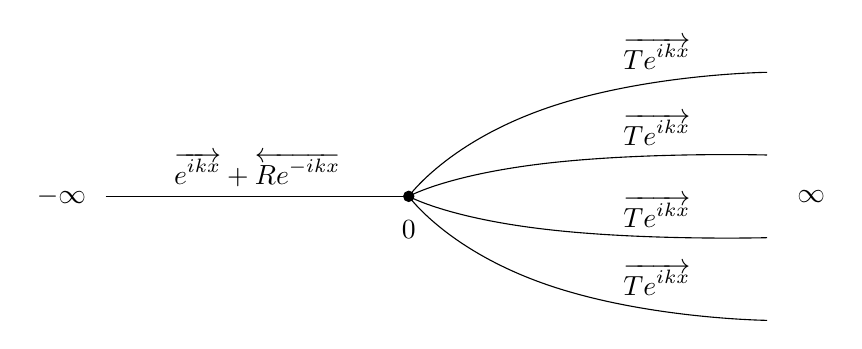
\begin{tikzpicture}[vertex/.style={draw,circle,minimum size=1.3mm,inner sep=0pt,outer sep=0pt,fill=black},scale=0.7]
    \draw (-5.5,0) -- (0,0);
    \node[vertex] at (0,0) {};
    \draw plot [smooth,tension=1] coordinates{(0,0) (2.5,1.6)  (6.5,2.25)};
    \draw plot [smooth,tension=1] coordinates{(0,0) (2.5,0.6)  (6.5,0.75)};
    \draw plot [smooth,tension=1] coordinates{(0,0) (2.5,-0.6) (6.5,-0.75)};
    \draw plot [smooth,tension=1] coordinates{(0,0) (2.5,-1.6) (6.5,-2.25)};
    \node[above] at (-2.75,0)   {$\overrightarrow{e^{ikx}}+\overleftarrow{Re^{-ikx}}$};
    \node at (4.5,2.6)  {$\overrightarrow{Te^{ikx}}$};
    \node[above] at (4.5,0.75)  {$\overrightarrow{Te^{ikx}}$};
    \node[above] at (4.5,-0.75) {$\overrightarrow{Te^{ikx}}$};
    \node at (4.5,-1.5) {$\overrightarrow{Te^{ikx}}$};
    \node at (-6.3,0) {$-\infty$};
    \node at (0,-0.6) {$0$};
    \node at (7.3,0) {$\infty$};
  \end{tikzpicture}
  \caption{Infinite star graph with one incoming wave being transmitted and reflected at the inner vertex.}
  \label{fig: scattering from infinite star graph}
\end{figure}

% We remain in the setting of the previous example, namely considering an infinite star graph of degree $d$.

Let us now consider a slightly different situation, where we have a wave incoming towards the vertex $v$ only on one of the edges edge, say $e_1$, the remaining edges are still identical. This should be thought of as physically approaching the graph at edge $e_1$ where one continuously sends in a stationary wave. We are then interested in how much of the wave gets transmitted via the inner vertex to the other edges, and how much of the wave gets reflected back on $e_1$. We thus write the general eigenfunctions on the $j$:th edge as
\[
  u_j(x) =
  \begin{cases}
    e^{ikx} + Re^{-ikx}, & j = 0 \\
    Te^{ikx}, & 1 \le j \le d-1,
  \end{cases}
\]
where we have chosen the normalized coefficient $1$ for the incoming wave, any other choice would simply rescale the solutions. The coefficients $R$ and $T$ are reflection and transmission coefficients, and the corresponding probabilities $\abs{R}^2$ and $\abs{T}^2$ should be interpreted as the fraction, ``how much'', of the wave that gets reflected and transmitted, respectively. It is not a priori clear that the eigenfunctions $u_j$ for $1 \le j \le d-1$ coincide, this was for instance not the case for the finite star graph, we will however see that this is the case here. With the parametrization of the edges as indicated by figure~\ref{fig: scattering from infinite star graph} we can write the standard matching conditions at the inner vertex as
\[
  \begin{dcases}
    u_j(x) = u_{j'}(x) \quad \text{for all } j, j' \\
    \sum_{j=0}^{d-1} \partial u_j(x) = 0
  \end{dcases}
  \iff
  \begin{dcases}
    R+1 = T_j, \quad j = 1, \ldots, d-1 \\
    -ik(1-R)+ik\sum_{j=1}^{d-1} T_j = 0.
  \end{dcases}
\]
From the first equation we immediately have all $T_j = T$ for some $T$ and the system is easily solved
\[
  \begin{cases}
    T = 2/d \\
    R = -1 + 2/d.
  \end{cases}
\]
We see that the spectrum is continuous, the reflection and transmission coefficients $R$ and $T$ depend only on the degree $d$ of the star graph, there is no dependence $k$. This will always be the case for scattering phenomena, more generally this always holds when a quantum mechanical particle not influenced by any potential --- recall that a finite edge can be regarded as a potential, c.f.\ example \label{ex: particle in a box}.

The probability that the wave will get reflected is given by
\[
  \abs{R}^2 = \left(\frac{d-2}{d}\right)^2
\]
which is monotonically increasing in $d$ and approaches $1$. This is a rather counterintuitive observation: when there are more edges for the wave to get transmitted through, the probability of the wave getting reflected increases. Since we are considering scattering phenomena, we can verify that this solution preserves probabilities, as discussed in section~\ref{sec: scattering phenomena}. The incoming wave was normalized and we have one reflected wave and $(d-1)$ transmitted waves. Hence we get
\[
  (d-1)T^2 + R^2 = (d-1)\frac{4}{d^2} + \frac{4}{d^2} - \frac{4}{d} + 1 = 1,
\]
showing that the probability is conserved after scattering at the vertex.



\section{Edge parametrization and interference}\label{sec: edge parametrization}

Before we proceed we will take a closer look at edge parametrization and consider how edge parametrization affects our calculations, in particular in relation to scattering. As we will see, in general we are free to parametrize the edges however we want without affecting the graph in any distinguishable way (see in particular example~\ref{ex: phase shift due to edge parametrization}). The important characteristics of an edge is its length, and of course which vertices it is connected to.

Typically one chooses a parametrization of an edge with length $\ell$ such that $0 \le x \le \ell$, this is convenient both because $u(0)$ is particularly easy to work with, and that $\ell$ then enters naturally when working with the matching conditions. When the graph is considered to be a medium through which a wave propagates, it can be
natural to use a continuous parametrization as illustrated in figure~\ref{fig: edge parametrization}.

\begin{figure}[h]
  \centering
  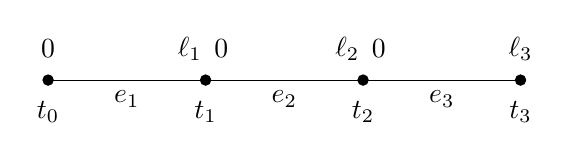
\begin{tikzpicture}[vertex/.style={draw,circle,minimum size=1.3mm,inner sep=0pt,outer sep=0pt,fill=black},scale=2]
    \draw (0,0) -- (3,0);
    \node[vertex] at (0,0) {};
    \node[vertex] at (1,0) {};
    \node[vertex] at (2,0) {};
    \node[vertex] at (3,0) {};

    \node at (0,0.2) {$0$};
    \node at (0.9,0.2) {$\ell_1$};
    \node at (1.1,0.2) {$0$};
    \node at (1.9,0.2) {$\ell_2$};
    \node at (2.1,0.2) {$0$};
    \node at (3,0.2) {$\ell_3$};

    \node at (0,-0.2) {$t_0$};
    \node at (1,-0.2) {$t_1$};
    \node at (2,-0.2) {$t_2$};
    \node at (3,-0.2) {$t_3$};

    \node at (0.5,-0.12) {$e_1$};
    \node at (1.5,-0.12) {$e_2$};
    \node at (2.5,-0.12) {$e_3$};
  \end{tikzpicture}
  \caption{Two types of edge parametrization. Natural edge parametrization above and continuous parametrization below, where $t_n = \sum_{j=1}^{n} \ell_j$.}
  \label{fig: edge parametrization}
\end{figure}

\begin{example}\label{ex: phase shift due to edge parametrization}
  We now consider how a discontinuous parametrization introduces a phase shift, and show that it is not of physical significance. Consider a quantum graph with standard matching conditions consisting of two semi-infinite edges with parametrization $(-\infty,0]$ and $[a,\infty)$, as illustrated in figure~\ref{fig: discontinuous parametrization of the line}.
  \begin{figure}[h]
    \centering
    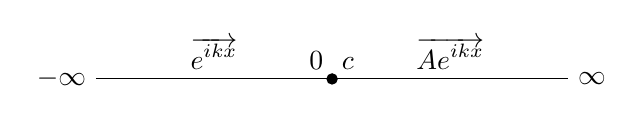
\begin{tikzpicture}[vertex/.style={draw,circle,minimum size=1.3mm,inner sep=0pt,outer sep=0pt,fill=black},scale=2]
      \draw (0,0) -- (3,0);
      \node[vertex] at (1.5,0) {};
      \node[left] at (0,0) {$-\infty$};
      \node[right] at (3,0) {$\infty$};
      \node[above] at (1.4,0) {$0$};
      \node[above] at (1.6,0) {$c$};
      \node[above] at (0.75,0) {$\overrightarrow{e^{ikx}}$};
      \node[above] at (2.25,0) {$\overrightarrow{Ae^{ikx}}$};
    \end{tikzpicture}
    \caption{Discontinuous edge parametrization introduces a phase shift $A = e^{-ika}$ of the wave, to ensure continuity.}
    \label{fig: discontinuous parametrization of the line}
  \end{figure}
  From the continuity condition we directly have $1 = Ae^{ikc}$ hence $A = e^{-ikc}$, the condition on the derivative gives nothing more. The discontinuous parametrization can be seen as the edges not being aligned, however the standard matching conditions require the wave to be continuous and the jump of the wave is compensated by shifting the wave by a phase $ka$ corresponding to the apparent separation of the edges due to the parametrization.

  We now show that this effect is not of physical significance. Consider the same graph but with an additional edge of length $\ell$ inserted between the two semi-infinite edges, parametrize it by $x \in [a,b]$ where $a < b < c$. On the middle edge we then have the wave $e^{-ika}e^{ikx}$ by the argument above. Let the wave on the right edge be $Te^{ikx}$, then by the continuity condition at the right vertex we have $e^{-ika}e^{ikb} = Te^{ikc}$. Hence $T = e^{ik\big((b-a)-c\big)}$, showing that only the length $b-a = \ell$ of the middle edge comes into play and that we are free to choose the parametrization as we like.
  Furthermore, recall that it is only the squared absolute value of the probability amplitude that can be directly measured.
\end{example}

From the above example we see that there is an interplay between introducing a phase shift and discontinuous edge parametrization. The situation is more interesting if we have two sources as we shall see in the next example.
% if two waves with different phase join up on one edge we get interference due to the phase shift of the two waves.

\begin{example}
  Consider an infinite star graph with 3 edges $e_1, e_2$ and $e_3$, along the edges $e_1$ and $e_2$ we send in waves (of the same energy $\lambda = k^2$), each with the amplitude $A_1$ and $A_2$ respectively, cf.\ figure~\ref{fig: infinite star graph interference}. Due to normalization we have $\abs{A_1}^2+\abs{A_2}^2=1$.
  % From normalization we then know $\abs{A_1}^2+\abs{A_2}^2 = 1$.
  \begin{figure}[h]
    \centering
    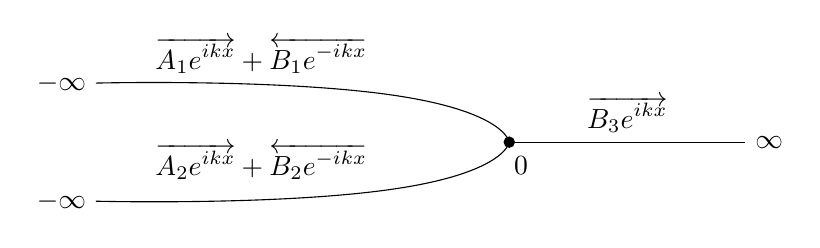
\begin{tikzpicture}[vertex/.style={draw,circle,minimum size=1.3mm,inner sep=0pt,outer sep=0pt,fill=black},scale=1.5]
      \node[vertex] at (0,0) {};
      \node at (0.1,-0.2) {$0$};
      \draw (0,0) -- (2,0);
      \draw plot [smooth,tension=1] coordinates{(-3.5,0.5) (-1,0.4) (0,0)};
      \draw plot [smooth,tension=1] coordinates{(-3.5,-0.5) (-1,-0.4) (0,0)};
      \node[above] at (-2.1,0.5) {$\overrightarrow{A_1e^{ikx}}+\overleftarrow{B_1e^{-ikx}}$};
      \node[above] at (-2.1,-0.4) {$\overrightarrow{A_2e^{ikx}}+\overleftarrow{B_2e^{-ikx}}$};
      \node[above] at (1,0) {$\overrightarrow{B_3e^{ikx}}$};
      \node[left] at (-3.5,0.5) {$-\infty$};
      \node[left] at (-3.5,-0.5) {$-\infty$};
      \node[right] at (2,0) {$\infty$};
    \end{tikzpicture}
    \caption{Infinite star graph with two wave sources causing interference.}
    \label{fig: infinite star graph interference}
  \end{figure}
  From section~\ref{sec: scattering from infinite star graph} we know that for each wave source we have transmission coefficient $T=A2/d$ and reflection coefficient $R=A(2/d-1)$ where $A$ is the amplitude of the incoming wave and $d$ is the degree of the star graph, 3 in our case. Note that the wave with coefficient $B_3$ contains transmission from both sources and $B_1$ contains transmission from $A_2$ and reflection from $A_1$ and vice versa. Hence we have
  \begin{align*}
    B_1 &= \frac{1}{3}\big(2A_1-A_2\big) \\
    B_2 &= \frac{1}{3}\big(2A_2-A_1\big) \\
    B_3 &= \frac{2}{3}\big(A_1+A_2\big).
  \end{align*}

  Without loss of generality we can write $A_j = e^{i\theta_j}a_j, j=1,2$ where $\theta_j$ and $a_j$ are real. The total transition probability is then given by
  \begin{align*}
    \abs{B_3}^2 &=
    \frac{4}{9}\big(A_1+A_2\big)\overline{\big(A_1+A_2\big)} \\ &=
    \frac{4}{9}\big(e^{i\theta_1}a_1+e^{i\theta_2}a_2\big)\big(e^{-i\theta_1}a_1+e^{-i\theta_2}a_2\big) \\ &=
    \frac{4}{9}\g{\underbrace{a_1^2+a_2^2}_{=1}+a_1a_2\g{e^{i(\theta_2-\theta_1)}+e^{-i(\theta_2-\theta_1)}}} \\ &=
    \frac{4}{9}\big(1+2a_1\sqrt{a_1^2-1}\cos (\theta_2-\theta_1)\big),
  \end{align*}
  where we in the last step used that $a_1^2+a_2^2=1$ due to normalization.
  This transition probability depends on how the initial wave is distributed between edge $e_1$ and $e_2$, in particular $\abs{B_3}^2$ is maximized for $a_1=1/\sqrt{2}$, i.e.\ $\abs{A_1}^2+\abs{A_2}^2=1/2$, equal amounts on both edges, for which $\abs{B_3}^2=8/9$ if the phases $\theta_1$ and $\theta_2$ coincide.

  We shall now see that by introducing a discontinuous edge parametrization for say edge $e_2$, that is, the right end-point will correspond to $x = a \ne 0$, will lead to interference. Indeed, as we have seen, such a parametrization is the same as adding a phase factor $ak$ to the amplitude of the wave, that is $A_2 \to e^{ika}A_2$, giving
  \begin{align*}
    \abs{B_3}^2 &=
    \frac{4}{9}\big(A_1+e^{ika}A_2\big)\overline{\big(A_1+e^{ika}A_2\big)} \\ &=
    \frac{4}{9}\big(e^{i\theta_1}a_1+e^{i(\theta_2+ka)}a_2\big)\big(e^{-i\theta_1}a_1+e^{-i(\theta_2+ka)}a_2\big) \\ &=
    \frac{4}{9}\g{a_1^2+a_2^2+a_1a_2\g{e^{i(ka+\theta_2-\theta_1)}+e^{-i(ka+\theta_2-\theta_1)}}} \\ &=
    \frac{4}{9}\g{a_1^2+a_2^2+2a_1a_2\cos(ka+\theta_2-\theta_1)} \\ &=
    \frac{4}{9}\g{1+2a_1\sqrt{a_1^2-1}\cos(ka+\theta_2-\theta_1)}
  \end{align*}
  and we see that we get an energy-dependent interference from the factor $\cos(ka+\theta_2-\theta_1)$.

  This example illustrates that when dealing with multiple wave sources one must make sure not to introduce interfering phase factors from parametrization. Note however, this is not in violation with the more general discussion in that parametrization can be chosen freely, since the change of parametrization here discussed is actually more than just an alternative parametrization, as we record in the following lemma.
\end{example}

\begin{lemma}
  As shown in the above two examples, using a discontinuous parametrization with distance $a$ introduces a phase shift $e^{ika}$. This phase shift is significant only if there are two wave sources, in which case the discontinuous edge parametrization should be understood as changing the length of one source edge. Thereby giving a different graph, which exhibits interference phenomena.
\end{lemma}



\section{Radial quantum tree graphs}\label{sec: radial graphs}

This section generalizes section~\ref{sec: scattering from infinite star graph} and serve as an introduction to chapter~\ref{sec: snowflake}. We will be interested in how the reflection $R$ from a radial quantum tree graph depends on the energy of the wave and the geometry of the graph. We begin with the definition.

\begin{definition}\label{def: radial quantum tree graph}
  A \emph{radial quantum tree graph} $\Gamma$ is a quantum graph where the underlying metric graph is a radial tree, meaning that the following properties are satisfied:
  \begin{itemize}
    \item The graph is a \emph{tree}, i.e\ it is connected and has no cycles.
    \item The graph is \emph{radial}, i.e\ all properties (such as edge length) of the graph depend only on the distance from one vertex, the root vertex.
  \end{itemize}
  For such graphs we define the following terminology.
  \begin{itemize}
    \item The $n$:th \emph{generation} is the set of all edges being $n-1$ edges away from the root edge. Note that, since the graph is radial, all edges belonging to the same generation has the same length.
    \item The \emph{branching number} of the $n$:th generation is the number $b \ge 1$ of edges connected to each edge in generation $n-1$. For the first generation the branching number is simply the number of edges in that generation.
    \item A \emph{branch} is a subgraph of $\Gamma$ that is itself a radial quantum tree graph.
  \end{itemize}
  The notation is illustrated in figure~\ref{fig: radial quantum tree graph} where a radial quantum tree graph with 3 generations is depicted.
\end{definition}

\begin{figure}[h]
  \centering
  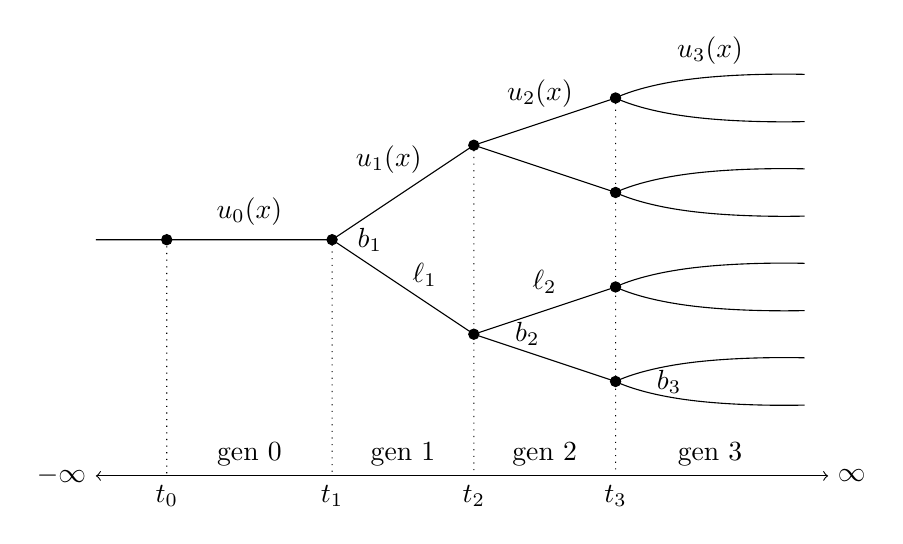
\begin{tikzpicture}[vertex/.style={draw,circle,minimum size=1.3mm,inner sep=0pt,outer sep=0pt,fill=black},scale=1.2]
    \path
      (0.25,0) node[vertex] (0)   {}
      (2,0)    node[vertex] (p0)  {}
      (3.5,1)  node[vertex] (p11) {}
      (3.5,-1) node[vertex] (p12) {}
      (5,1.5)  node[vertex] (p21) {}
      (5,0.5)  node[vertex] (p22) {}
      (5,-0.5) node[vertex] (p23) {}
      (5,-1.5) node[vertex] (p24) {};
    \node[right=0.2cm] at (p0) {$b_1$};
    \node[right=0.4cm] at (p12) {$b_2$};
    \node[right=0.4cm] at (p24) {$b_3$};
    \node[above right] at (2.75,-0.6) {$\ell_1$};
    \node at (4.25,-0.45) {$\ell_2$};
    \node at (1.125,0.3) {$u_0(x)$};
    \node at (2.6,0.85) {$u_1(x)$};
    \node at (4.2,1.55) {$u_2(x)$};
    \node at (6,2) {$u_3(x)$};
    \draw
      (-0.5,0) -- (0)
      (0)   -- (p0)
      (p0)  -- (p11)
      (p0)  -- (p12)
      (p11) -- (p21)
      (p11) -- (p22)
      (p12) -- (p23)
      (p12) -- (p24);
    \draw plot [smooth,tension=1] coordinates{(p21) (5.8,1.7) (7,1.75)};
    \draw plot [smooth,tension=1] coordinates{(p21) (5.8,1.3) (7,1.25)};
    \draw plot [smooth,tension=1] coordinates{(p22) (5.8,0.7) (7,0.75)};
    \draw plot [smooth,tension=1] coordinates{(p22) (5.8,0.3) (7,0.25)};
    \draw plot [smooth,tension=1] coordinates{(p23) (5.8,-0.7) (7,-0.75)};
    \draw plot [smooth,tension=1] coordinates{(p23) (5.8,-0.3) (7,-0.25)};
    \draw plot [smooth,tension=1] coordinates{(p24) (5.8,-1.7) (7,-1.75)};
    \draw plot [smooth,tension=1] coordinates{(p24) (5.8,-1.3) (7,-1.25)};
    \draw[dotted]
      (0.25,0) -- (0.25,-2.5)
      (p0)     -- (2,-2.5)
      (p11)    -- (3.5,-2.5)
      (p21)    -- (5,-2.5);
    \draw[<->] (-0.5,-2.5) -- (7.25,-2.5);
    \node[below] (t0) at (0.25,-2.5) {$t_0$};
    \node[below] (t1) at (2,-2.5) {$t_1$};
    \node[below] (t2) at (3.5,-2.5) {$t_2$};
    \node[below] (t3) at (5,-2.5) {$t_3$};
    \node[left]  (-infty) at (-0.5,-2.5) {$-\infty$};
    \node[right] (intfy) at (7.25,-2.5) {$\infty$};
    \node[above] at (1.125,-2.5) {gen 0};
    \node[above] at (2.75,-2.5) {gen 1};
    \node[above] at (4.25,-2.5) {gen 2};
    \node[above] at (6,-2.5) {gen 3};
  \end{tikzpicture}
  \caption{Radial quantum tree graph with semi-infinite edges in the final generation and a semi-infinite edge attached to the root edge.}
  \label{fig: radial quantum tree graph}
\end{figure}

% \begin{remark}[Notation]
%   Let $I_{j,k}$ denote the $k$:th interval on the $j$:th generation. The short-hand notation $I_j$ for $I_{j,1}$ will be convenient in section~\ref{sec:symmetry}. Let the left and right endpoints of $I_{j,k}$ be $x_{j,k}^0$ and $x_{j,k}^1$, respectively, with $x_j^0$ and $x_j^1$ as shorthand for $x_{j,1}^0$ and $x_{j,1}^1$, respectively.
% \end{remark}

\begin{remark}\label{rem: semi-infinite edges for scattering}
  Since we are considering scattering phenomena we require the edge $e_0$ to be semi-infinite. This edge $e_0$ should be thought of as our way in to the graph, the edge on which the incoming wave propagates. This is clearly not physically realizable, but such an edge is a good model for a source ``far away'' from the graph, where the source is not part of the graph. In particular a semi-infinite edge has only one end-point, allowing us to not have any matching conditions ``outside'' the graph being considered.

  Likewise we require the edges in the final generation to be semi-infinite. Otherwise the the entire wave necessarily gets reflected, indeed the wave has nowhere else to go. If we choose the parametrization so that $x=0$ at the vertex joining $e_0$ with the graph, we get precisely $R=1$.

  Finally, note that there is another possibility, namely that there is no last generation.

  Thus we will we will only consider radial quantum tree graphs with a semi-infinite edge attached to the root vertex, and semi-infinite edges attached at the last generation, or infinitely many generations.
\end{remark}

In this section we use a direct approach to study the reflection of radial quantum tree graphs, which will be a source of intuition and comparison to the results in chapter~\ref{sec: snowflake} where we consider a specific type of radial quantum tree graph of infinite number of generations.

In section~\ref{sec: scattering from infinite star graph} we have already studied radial graphs of one generation. We will now consider the reflection of a radial quantum tree graph with 2 generations.



\subsection{Reflection from 2 generations}\label{sec: 2 gen matrix}

Let the first generation have length $\ell_1$ and contain $b_1$ edges. The second generation contains $b_1b_2$ number of semi-infinite edges.

Since all edges belonging to the same generation are identical, we have that, for an incoming wave on the root edge $e_0$, the eigenfunctions of $L$ on the graph are
\begin{equation}
  u(x) = \begin{cases}
       e^{ikx} + Re^{-ikx}   & \text{generation 0} \\
    Ae^{ikx} + Be^{-ikx} & \text{generation 1} \\
    Te^{ikx}                 & \text{generation 2}.
  \end{cases}
\end{equation}
We are interested in how the coefficient $R$ depends on the properties of the graph, the coefficients $B$ and $A$ are intermediate reflection and transmission coefficients on the middle edge. By the radial structure of the graph, the matching conditions at each vertex belonging to the same generation will be identical. Hence the standard matching condition gives us the set of four equations
\begin{align}
  & \begin{cases}
    1+R = A+B \\
    -ik(1-R) + b_1 ik(A-B) = 0
  \end{cases} \\
  & \begin{cases}
    Ae^{ik\ell_1} + Be^{-ik\ell_1} = Te^{ik\ell_1} \\
    -ik(Ae^{ik\ell_1}-Be^{-ik\ell_1}) + b_2 ikTe^{ik\ell_1} = 0
  \end{cases}
\end{align}
where the first two equations come from the vertex connecting generation 0 and 1, while the last two equations come from any vertex connecting generations 1 and 2. This is a linear system of equations which we most conveniently represented as a matrix equation
\begin{equation}
  \begin{pmatrix}
    -1 & 1             & 1             & 0                \\
    1  & b_1           & -b_1          & 0                \\
    0  & e^{ik\ell_1}  & e^{-ik\ell_1} & -e^{ik\ell_1}    \\
    0  & -e^{ik\ell_1} & e^{-ik\ell_1} & b_2 e^{ik\ell_1}
  \end{pmatrix}
  \begin{pmatrix}
    R \\ A \\ B \\ T
  \end{pmatrix}
  =
  \begin{pmatrix}
    1 \\ 1 \\ 0 \\ 0
  \end{pmatrix}
\end{equation}
and solve for $R$ using using Cramer's rule, as follows
\begin{equation}\label{eq: 2gen R}
  \begin{aligned}
    R(k) &= \frac{
      \begin{vmatrix}
        1 & 1             & 1             & 0                \\
        1 & b_1           & -b_1          & 0                \\
        0 & e^{ik\ell_1}  & e^{-ik\ell_1} & -e^{ik\ell_1}    \\
        0 & -e^{ik\ell_1} & e^{-ik\ell_1} & b_2 e^{ik\ell_1}
      \end{vmatrix}
    }{
      \begin{vmatrix}
        -1 & 1             & 1             & 0                \\
        1  & b_1           & -b_1          & 0                \\
        0  & e^{ik\ell_1}  & e^{-ik\ell_1} & -e^{ik\ell_1}    \\
        0  & -e^{ik\ell_1} & e^{-ik\ell_1} & b_2 e^{ik\ell_1}
      \end{vmatrix}
    } \\
    &= -\frac{(b_1-1) (b_2+1)+(b_1+1) (b_2-1) e^{2 i k \ell_1}}{(b_1+1) (b_2+1)+(b_1-1) (b_2-1) e^{2 i k \ell_1}}.
  \end{aligned}
\end{equation}
We are not interested in the explicit expression for $T(k)$, since we can always calculate $\abs{T}^2$ from the relation $\abs{R}^2 + b_1b_2\abs{T}^2 = 1$.

Recall that for a one-generation radial tree the reflection amplitude was independent of the energy, for two generations we see that the situation is quite different. From the expression of $R$ we see that the reflection coefficient is periodic in $k$ with period $\pi/\ell_1$. This fact can be understood as coming from that all reflected components of the wave interfere constructively and destructively for different energies. However, note that this interference  In section~\ref{sec: scattering in the snowflake} we will consider such internal reflections and generalize the concept.

If we set one of the branching numbers $b_1$ or $b_2$ equal to 1, say $b_1=1$, then the graph effectively becomes a star graph of degree $b_2+1$ since the vertices of degree 2 can be removed, as we have seen in example \ref{ex: remove vertex smc}. Hence we expect to get back the result found in section~\ref{sec: scattering from infinite star graph}, at least up to some phase shift factor $e^{i\phi}$, which does not affect the reflection probability. For a star graph of degree $d$ we found the reflection coefficient to be $R = 2/d - 1$. With $b_1 = 1$ we have $d = b_2 + 1$ and the expression for $R(k)$ becomes
\[
  R(k) = - \frac{2(b_2-1)}{2(b_2+1)} e^{2ik\ell_1} = \left( \frac{2}{b_2+1} - 1 \right) e^{2ik\ell_1}
\]
similarly, for $b_2=1$ we get
\[
  R(k) = - \frac{(b_1-1)2}{(b_1+1)2} = \frac{2}{b_1+1} - 1.
\]
The phase shift emerges from that the choice of parametrization differs from that of section~\ref{sec: scattering from infinite star graph}, recall the discussion in section~\ref{sec: edge parametrization}.

We get a similar result by considering zero energy, that is $k=0$, for which we have
\[
  R(0) = -\frac{(b_1-1)(b_2+1)+(b_1+1)(b_2-1)}{(b_1+1)(b_2+1)+(b_1-1)(b_2-1)} = -\frac{b_1b_2-1}{b_2b_2+1} = \frac{2}{b_1b_2+1} - 1.
\]
This is precisely the reflection coefficient of a star graph of degree $d = b_1b_2 + 1$, where $b_1b_2$ is the number of edges in final generation. This can be interpreted as that the wave does not ``see'' the middle vertices when it has very low energy. In \cref{res: R(0)} we show that this holds also for graphs with higher number of generations. Since we have found $R(k)$ to be periodic for $n=2$ generations, with period $\pi/\ell_1$, we must have the same reflection for $k=n\pi/\ell_1$ where $n=1,2,3,\ldots$.

Let us now consider the reflection probability for general energies, namely $\abs{R(k)}^2$, it can be written as
%% See bottom of 2gen.nb.
\begin{equation}\label{eq: 2 gen reflection probability}
  \abs{R(k)}^2 = \frac{(b_1-b_2)^2 \sin ^2(k \ell_1)+(b_1 b_2-1)^2 \cos ^2(k \ell_1)}{(b_1+b_2)^2 \sin ^2(k \ell_1)+(b_1 b_2+1)^2 \cos ^2(k \ell_1)}.
\end{equation}
Evidently this expression is invariant when interchanging $b_1$ and $b_2$. This gives another interesting result:
\begin{theorem}\label{res: isoscattering graphs}
  Let $\Gamma$ be a radial quantum tree graph with two generations of edges and branching numbers $b_1$ and $b_2$. Construct $\widehat{\Gamma}$ by interchanging $b_1$ and $b_2$ in $\Gamma$. The probability of getting reflection from the two graphs $\Gamma$ and $\widehat{\Gamma}$ is identical, they graphs cannot be distinguished by measuring the probability of reflection from the root of the graphs.
\end{theorem}

From the derivative of the reflection probability,
\[
  \Dop{k} \abs{R(k)}^2 = -\frac{4 b_1 \left(b_1^2-1\right) b_2\left(b_2^2-1\right) \ell_1 \sin (2 k\ell_1)}{\left((b_1+b_2)^2 \sin ^2(k\ell_1)+(b_1 b_2+1)^2 \cos ^2(k\ell_1)\right)^2},
\]
we see that we get minimal or maximal reflection for $\sin 2k\ell_1 = 0$ that is $k = \frac{\pi}{2\ell}n$. For these values of $k$ we have
\begin{align}
  \abs{R\left(\frac{\pi}{2\ell_1}(2m)\right)}^2 &=
  \left(\frac{b_1b_2-1}{b_1b_2+1}\right)^2 = \left(\frac{1}{b_1b_2+1} - 1\right)^2 \\
  \abs{R\left(\frac{\pi}{2\ell_1}(2m+1)\right)}^2 &=
  \left(\frac{b_1-b_2}{b_1+b_2}\right)^2 = \left(\frac{2b_2}{b_1+b_2} - 1\right)^2. \label{eq: 2 gen reflection probability minimum}
\end{align}
It is clear that the former is the maxima and the latter is the minima. In figure~\ref{fig: 2 gen reflection} we plot $\abs{R(k)}^2$ as a function of $k\ell_1$ for different branching numbers.

\begin{figure}[h]
  \begin{subfigure}[t]{0.5\textwidth}
    \includegraphics[width=1\textwidth]{img/2gen_reflection_l=1_b1=3_b2=7}
    \caption{$b_1=7, b_2=3$}
  \end{subfigure}
  \begin{subfigure}[t]{0.5\textwidth}
    \includegraphics[width=1\textwidth]{img/2gen_reflection_l=1_b1=b2=4}
    \caption{$b_1=b_2=4$}
  \end{subfigure}
  \\
  \begin{subfigure}[t]{0.5\textwidth}
    \includegraphics[width=1\textwidth]{img/2gen_reflection_l=1_b1=500_b2=10}
    \caption{$b_1=500, b_2=10$}
  \end{subfigure}
  \begin{subfigure}[t]{0.5\textwidth}
    \includegraphics[width=1\textwidth]{img/2gen_reflection_l=1_b1=100_b2=100}
    \caption{$b_1=b_2=100$}
    \label{fig: 2 gen reflection gap}
  \end{subfigure}
  \caption{Reflection $\abs{R}^2$ from 2 generation radial quantum tree graph with inner edge length $\ell_1=1$ and varying branching numbers $b_1$ and $b_2$.}
  \label{fig: 2 gen reflection}
\end{figure}

Let us now consider what happens in the limiting case when one branching number grows large. As we have seen, $b_1$ and $b_2$ occurs symmetrically in the expression for $\abs{R}^2$. Hence we can without loss of generality keep $b_1$ fixed and let $b_2 \to \infty$, then from \eqref{eq: 2 gen reflection probability minimum} we see that the minimal reflection approaces 1, and thus $\abs{R} \to 1$ for all $k$. Similar to the case of the one generation radial quantum tree graph, we have the somewhat counterintuitive result that the probability of getting a reflection increases when the wave has more edges to propagate through. Keep in mind, though, that for $b_1 = b_2$ we always get zero reflection at the points $k = (2n+1)\pi/\ell_1, n = 1,2,3,\ldots$, but the interval for low reflection around these points gets smaller with increasing branching numbers, cf.\ figure~\ref{fig: 2 gen reflection gap}.

To continue this process for an arbitrary number $n$ of generations is unwieldy because one needs to calculate the determinant of a $2n \times 2n$ matrix. Instead, we will in the following chapter develop another method which makes the problem more tractable, and furthermore also gives a better insight into the scattering inside the graph.



% \section{Reflection from radial graphs with $n$ generations}

% General solutions to $Lu=u$ are
% \begin{equation}
%   \psi_j(x) = T_je^{ikx}+R_je^{-ikx}
% \end{equation}
% where $0\leq j\leq n$ is the generation number and $T_0=1, R_n=0$. The standard matching conditions give the system of equations
% \begin{equation}
%   \begin{dcases}
%     \psi_{j-1}(t_j) = \psi_j(t_j) \\
%     -\frac{d}{dx}\psi_{j-1}(t_j) + b_j\frac{d}{dx}\psi_j(t_j) = 0
%   \end{dcases}
%   \quad 1\leq j\leq n
% \end{equation}
% That is
% \begin{equation}
%   \begin{aligned}
%     % j=1: & \begin{cases}
%     %   e^{ikt_j} + R_{j-1} e^{-ikt_j} = T_j e^{ikt_j} + R_j e^{-ikt_j} \\
%     %   -ik(e^{ikt_j} - R_{j-1} e^{-ikt_j}) + b_j ik (T_j e^{ikt_j} - R_j e^{-ikt_j}) = 0
%     % \end{cases}\\
%     % 2\leq j\leq n-1: &
%     \begin{cases}
%       T_{j-1} e^{ikt_j} + R_{j-1} e^{-ikt_j} = T_j e^{ikt_j} + R_j e^{-ikt_j} \\
%       -ik(T_{j-1} e^{ikt_j} - R_{j-1} e^{-ikt_j}) + b_j ik (T_j e^{ikt_j} - R_j e^{-ikt_j}) = 0
%     \end{cases} \\
%     % j=n: & \begin{cases}
%     %   T_{j-1} e^{ikt_j} + R_{j-1} e^{-ikt_j} = T_j e^{ikt_j} \\
%     %   -ik(T_{j-1} e^{ikt_j} - R_{j-1} e^{-ikt_j}) + b_j ik T_j e^{ikt_j} = 0.
%     % \end{cases}
%   \end{aligned}
% \end{equation}
% As a matrix equation for 3 generations
% \begin{equation}
%   \begin{pmatrix}
%     -e^{-ikt_0}  & e^{ikt_0}      & e^{-ikt_0}       & 0              & 0                & 0             \\
%     ike^{-ikt_0} & b_0ike^{ikt_0} & -b_0ike^{-ikt_0} & 0              & 0                & 0             \\
%     0            & -e^{ikt_1}     & -e^{-ikt_1}      & e^{ikt_1}      & e^{-ikt_1}       & 0             \\
%     0            & -ike^{ikt_1}   & ike^{-ikt_1}     & b_1ike^{ikt_1} & -b_1ike^{-ikt_1} & 0             \\
%     0            & 0              & 0                & -e^{ikt_2}     & e^{ikt_2}        & e^{-ikt_2}    \\
%     0            & 0              & 0                & -e^{ikt_2}     & -b_2e^{ikt_2}    & b_2e^{-ikt_2} \\
%   \end{pmatrix}
%   \begin{pmatrix}
%     R \\ A \\ B \\ T_2 \\ R_2 \\ T
%   \end{pmatrix}
%   =
%   \begin{pmatrix}
%     e^{ikt_0} \\ ike^{ikt_0} \\ 0 \\ 0 \\ 0 \\ 0
%   \end{pmatrix}.
% \end{equation}


% Some observations

% \begin{itemize}
%   \item For 3 generations with equal edge lengths $\ell$ and equal branching numbers $m$ we get zero reflection iff
%   \begin{equation}
%     \cos 2k\ell = -\frac{1+m^2}{(1+m)^2}
%   \end{equation}
%   \item For any number of generations with equal length and branching number it appears to always be possible to get zero reflection.
%   \item With $m=2$ and 3 generations, zero reflection is given by at least $\ell_1=2\ell_2$ and $\ell_1=7\ell_2$, and symmetric between $\ell_1$ and $\ell_2$.
%   \item For 3 generations with equal branching number, $|R|^2$ is symmetric between the lengths.
% \end{itemize}


% \section{Minimal average reflection}

